%%%%%%%%%%%%%%%%%%%%%%%%%%%%%%%%%%%%%%%%%
% Beamer Presentation
% LaTeX Template
% Version 1.0 (10/11/12)
%
% This template has been downloaded from:
% http://www.LaTeXTemplates.com
%
% License:
% CC BY-NC-SA 3.0 (http://creativecommons.org/licenses/by-nc-sa/3.0/)
%
%%%%%%%%%%%%%%%%%%%%%%%%%%%%%%%%%%%%%%%%%

%----------------------------------------------------------------------------------------
%	PACKAGES AND THEMES
%----------------------------------------------------------------------------------------

\documentclass[greek]{beamer}

\mode<presentation> {

% The Beamer class comes with a number of default slide themes
% which change the colors and layouts of slides. Below this is a list
% of all the themes, uncomment each in turn to see what they look like.

%\usetheme{default}
%\usetheme{AnnArbor}
%\usetheme{Antibes}
%\usetheme{Bergen}
\usetheme{Berkeley}
%\usetheme{Berlin}
%\usetheme{Boadilla}
%\usetheme{CambridgeUS}
%\usetheme{Copenhagen}
%\usetheme{Darmstadt}
%\usetheme{Dresden}
%\usetheme{Frankfurt}
%\usetheme{Goettingen}
%\usetheme{Hannover}
%\usetheme{Ilmenau}
%\usetheme{JuanLesPins}
%\usetheme{Luebeck}
%\usetheme{Madrid}
%\usetheme{Malmoe}
%\usetheme{Marburg}
%\usetheme{Montpellier}
%\usetheme{PaloAlto}
%\usetheme{Pittsburgh}
%\usetheme{Rochester}
%\usetheme{Singapore}
%\usetheme{Szeged}
%\usetheme{Warsaw}

% As well as themes, the Beamer class has a number of color themes
% for any slide theme. Uncomment each of these in turn to see how it
% changes the colors of your current slide theme.

%\usecolortheme{albatross}
%\usecolortheme{beaver}
%\usecolortheme{beetle}
%\usecolortheme{crane}
\usecolortheme{dolphin}
%\usecolortheme{dove}
%\usecolortheme{fly}
%\usecolortheme{lily}
%\usecolortheme{orchid}
%\usecolortheme{rose}
%\usecolortheme{seagull}
%\usecolortheme{seahorse}
%\usecolortheme{whale}
%\usecolortheme{wolverine}

%\setbeamertemplate{footline} % To remove the footer line in all slides uncomment this line
%\setbeamertemplate{footline}[page number] % To replace the footer line in all slides with a simple slide count uncomment this line

%\setbeamertemplate{navigation symbols}{} % To remove the navigation symbols from the bottom of all slides uncomment this line
}
\usepackage[utf8]{inputenc} % Required for inputting international characters
\usepackage[T1]{fontenc} % Output font encoding for international characters
\usepackage{palatino} % Use the Palatino font by default

\usepackage[cm-default]{fontspec}
\usepackage{enumerate}
\usepackage{amsmath}
\usepackage{ragged2e}
\usepackage{float}
% \usepackage{polyglossia}

\usepackage{graphicx} % Allows including images
\usepackage{booktabs} % Allows the use of \toprule, \midrule and \bottomrule in tables
\usepackage{listings}
\usepackage{color}

\usepackage{minted}
\usepackage[greek]{babel}
\usepackage{xgreek} 

\setromanfont{FreeSerif}
\setsansfont{FreeSans}
\setmonofont{FreeMono}

\definecolor{darkgray}{gray}{0.1}
\definecolor{lbcolor}{rgb}{0.9,0.9,0.9}
\definecolor{mauve}{rgb}{0.48,0,0.72}

\lstset{
  language=C++,                   % choose the language of the code
  backgroundcolor=\color{white},  % choose the background color. You must add \usepackage{color}
  basicstyle=\ttfamily,
  numberstyle=\color{mauve}\ttfamily,
  keywordstyle=\color{blue}\ttfamily,
  stringstyle=\color{red}\ttfamily,
  commentstyle=\color{green}\ttfamily,
  frame=single,
  showspaces=false,               % show spaces adding particular underscores
  showstringspaces=false,         % underline spaces within strings
  showtabs=false,                 % show tabs within strings adding particular underscores
  tabsize=2,                      % sets default tabsize to 2 spaces
  captionpos=b,                   % sets the caption-position to bottom
  breaklines=false,                % sets automatic line breaking
  breakatwhitespace=false,         % sets if automatic breaks should only happen at whitespace
  title=\lstname,                 % show the filename of files included with \lstinputlisting;
}

\usepackage[bibstyle=alphabetic, citestyle=alphabetic]{biblatex}
\addbibresource[datatype=bibtex]{../example.bib}   


\AtBeginSection[]{
  \begin{frame}
  \vfill
  \centering
  \begin{beamercolorbox}[sep=8pt,center,shadow=true,rounded=true]{title}
    \usebeamerfont{title}\insertsectionhead\par%
  \end{beamercolorbox}
  \vfill
  \end{frame}
}

%----------------------------------------------------------------------------------------
%	TITLE PAGE
%----------------------------------------------------------------------------------------

\title[Vertex Cover]{Vertex Cover Problem} 
\author{Δημήτρης Δήμου}
\institute[UP]
{
Τμήμα Ηλεκτρολόγων Μηχανικών και Τεχνολογίας Υπολογιστών\\
Πανεπιστήμιο Πατρών\\ 
\medskip
\textit{mijuomij@gmail.com}
}
\
\date{\today} 

\begin{document}

\begin{frame}
\titlepage 
\end{frame}

\begin{frame}
\frametitle{Περιεχόμενα} 
\tableofcontents 
\end{frame}

%----------------------------------------------------------------------------------------
%	PRESENTATION SLIDES
%----------------------------------------------------------------------------------------

%------------------------------------------------
%------------------------------------------------
%------------------------------------------------

\section{Set Cover Problem} 


%------------------------------------------------
%------------------------------------------------

\subsection{Διατύπωση}

%------------------------------------------------

\begin{frame}
\frametitle{Διατύπωση}
Set cover:\\
Δεδομένου ενός σύμπαντος $U$ αποτελούμενο από $n$ στοιχεία κι ενός συνόλου από υποσύνολα του $U$, $S = \{S_1,...,S_k\}$ τέτοια ώστε η ένωσή τους να είναι το σύνολο $U$, βρες το ελάχιστο υποσύνολο του $S$ που καλύπτει όλα τα στοιχεία του $U$.\\\
Παράδειγμα:\\
Έστω το σύμπαν $U = \{1, 2, 3, 4 ,5\}$ και η συλλογή από υποσύνολα του $S=\{\{1,2,3\},\{2,4\},\{3,4\},\{4,5\}\}
$. Η ένωση των στοιχείων του $S$ καλύπτει το $U$. H ελάχιστη συλλογή υποσυνόλων του $S$ που καλύπτει το $U$ είναι τα : $\{\{1,2,3\},\{4,5\}\}$.
\end{frame}

%------------------------------------------------

\subsection{NP-πληρότητα}

%------------------------------------------------
%------------------------------------------------

\begin{frame}
\frametitle{NP-πληρότητα}
To set cover decision problem είναι ένα από τα 21 NP-πλήρης προβλήματα του Karp. Αυτό σημαίνει ότι ανήκει στην κλάση NP και στην κλάση NP-hard. Αυτό οδήγησε στην ανάπτυξη διάφορων προσεγγιστικών αλγορίθμων για την επίλυση του προβλήματος αυτού.
\end{frame}

%------------------------------------------------
%------------------------------------------------

\subsection{Λύσεις}

%------------------------------------------------

\begin{frame}
\frametitle{Πρόβλημα ακέραιου προγραμματισμού}
Το minimum set cover problem μπορεί να διατυπωθεί ως το ακόλουθο πρόβλημα ακέραιου προγραμματισμού

$$min\{\displaystyle\sum_{S\in{\mathcal{S}}} x_S\}$$ 
\centerline{subject to}
$$\displaystyle\sum_{S:e\in{\mathcal{S}}} x_S \geq{1}, \quad \forall e \in{\mathcal{U}}$$
$$ x_S \in{\{0, 1\}}$$
\end{frame}

%------------------------------------------------

\begin{frame}
\frametitle{Χαλάρωση προβλήματος ακέραιου προγραμματισμού}
$$min\{\displaystyle\sum_{S\in{\mathcal{S}}} x_S\}$$ 
\centerline{subject to}
$$\displaystyle\sum_{S:e\in{\mathcal{S}}} x_S \geq{1}, \quad \forall e \in{\mathcal{U}}$$
$$ x_S \in{[0, 1]}$$\\

integrality gap: το πολύ $\log(n)$\\
approximation factor: $\log(n)$
\end{frame}

%------------------------------------------------

\begin{frame}
\frametitle{Άπληστος αλγόριθμος}
Αλγόριθμος:
\begin{enumerate}
\item $ C \leftarrow \emptyset$
\item While $ C \neq {\mathcal{U}} $ do
\begin{enumerate}
\item Find the set whose cost effectiveness is smallest, say $S_i$. \\
			Let $a = \frac{c(S_i)}{|S_i-C|}$. \\
			Pick $S_i$ and $\forall e \in{S_i - C}$, set $price(e) = a$.
\item $C \leftarrow S_i \cup C$
\end{enumerate}
\item Output $C$
\end{enumerate}
\end{frame}

%------------------------------------------------

\begin{frame}
\frametitle{Hitting Set}
Αν σε έναν διμερή γράφο το ένα σύνολο κόμβων ${\mathcal{U}}$ αντιπροσωπεύει τα υποσύνολα ${\mathcal{S}}$ του σύμπαντος, το άλλο σύνολο κόμβων ${\mathcal{V}}$ αντιπροσωπεύει τα στοιχεία του σύμπαντος και οι ακμές αντιπροσωπεύουν την συμπερίληψη ενός στοιχείου σε ένα σύνολο τότε βρίσκουμε τον ελάχιστο αριθμό κόμβων του συνόλου ${\mathcal{U}}$ που καλύπτει όλους τους κόμβους του συνόλου ${\mathcal{V}}$.
\end{frame}

%------------------------------------------------
%------------------------------------------------
%------------------------------------------------

\section{Vertex cover problem}

%------------------------------------------------
%------------------------------------------------

\subsection{Διατύπωση}

%------------------------------------------------

\begin{frame}
\frametitle{Διατύπωση}
Το vertex cover $V'$ ενός μη κατευθυντικού γράφου $G=(V,E)$ είναι ένα υποσύνολο του $V$ τέτοιο ώστε:
$$\forall uv \in{E} \Rightarrow u \in{V'} \lor v \in{V'}$$
Ένα τέτοιο σύνολο λέμε ό τι καλύπτει τις ακμές του $G$. Το ελάχιστο vertex cover ενός γράφου $G$ είναι το σύνολο $V'$ με τον μικρότερο αριθμό στοιχείων.
\end{frame}

%------------------------------------------------

\begin{frame}
\frametitle{Παραδείγματα}
\begin{figure}[H]
\caption{Vertex cover}
\centering
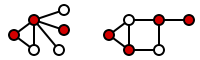
\includegraphics[width=0.6\textwidth]{Figures/vert_cover.png}\centering
\end{figure}

\begin{figure}[H]
\caption{Minimum vertex cover}
\centering
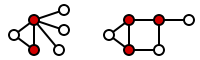
\includegraphics[width=0.6\textwidth]{Figures/min_vert_cover.png}\centering
\end{figure}
\end{frame}

%------------------------------------------------
%------------------------------------------------

\subsection{NP-πληρότητα}

%------------------------------------------------

\begin{frame}
\frametitle{NP-πληρότητα}
Και αυτό το πρόβλημα είναι NP-πλήρες και μπορεί να αναχθεί από το 3-SAT ή το Clique πρόβλημα.
Με εξαντλητική αναζήτηση η λύση δίνεται σε χρόνο $2^{k}n^{O(1)}$ το οποίο κάνει το πρόβλημα fixed-parameter tractable.
\end{frame}

%------------------------------------------------
%------------------------------------------------

\subsection{Λύσεις}

%------------------------------------------------

\begin{frame}
\frametitle{Πρόβλημα ακέραιου προγραμματισμού}
Το minimum vertex cover problem μπορεί να διατυπωθεί ως το ακόλουθο πρόβλημα ακέραιου προγραμματισμού

$$min\{\displaystyle\sum_{u\in{V}} c(v)x_v\}$$ 
\centerline{subject to}
$$x_u + x_v \geq{1}, \quad \forall (u, v) \in{E}$$
$$ x_v \in{\{0, 1\}} \quad \forall v \in{V}$$
\end{frame}

%------------------------------------------------

\begin{frame}
\frametitle{Χαλάρωση προβλήματος ακέραιου προγραμματισμού}

$$min\{\displaystyle\sum_{u\in{V}} c(v)x_v\}$$ 
\centerline{subject to}
$$x_u + x_v \geq{1}, \quad \forall (u, v) \in{E}$$
$$ x_v \in [0,1], \quad \forall v \in{V}$$
\end{frame}

%------------------------------------------------

\begin{frame}
\frametitle{Integrality gap}
Integrality gap:
$$\sup_{I} \frac{OPT(I)}{OPT_f(I)}$$\\

Το integrality gap του παραπάνω προβλήματος είναι $2$ οπότε η χαλάρωση του δίνει έναν factor-$2$ προσεγγιστικό αλγόριθμο. 
\end{frame}

%------------------------------------------------

\begin{frame}
\frametitle{Half-integrality}
Kάθε λύση ακραίου σημείου είναι half-integral δηλαδή $x_v \in{\{0, \frac{1}{2}, 1\}} \quad \forall x_v \in V'$ \cite{AppAlg}.
\end{frame}

%------------------------------------------------

\begin{frame}
\frametitle{Προσεγγιστικοί αλγόριθμοι}
Αλγόριθμος:
\begin{enumerate}
\item $ V' \leftarrow \emptyset $
\item $ E' \leftarrow E$
\item While $ E' \neq {\emptyset} $ do
\begin{enumerate}[a)]
\item let (u, v) be an arbitrary edge of $E'$
\item $V' \leftarrow V' \cup \{u,v\}$
\item remove from $E'$ every edge incident on either u or v 
\end{enumerate}
\item Output $V'$
\end{enumerate}
\end{frame}

\begin{frame}
\frametitle{Προσεγγιστικοί αλγόριθμοι}
Ο αλγόριθμος αυτός τρέχει σε χρόνο $O(|V| + |E|)$\cite{IntAlg}. Όσον αφορά τον παράγοντα προσέγγγισης του αλγορίθμου φαίνεται εύκολα ότι για το σύνολο των ακμών που επιλέγονται στο βήμα $\alpha')$ ισχύει 
$$|V^{*}| \geq |A|$$ 
αφού το σύνολο $Α$ δεν περιέχει προσκείμενες ακμές και επειδή το σύνολο $V'$ που επιστρέφει ο αλγόριθμος περιέχει και τις δυο κορυφές των ακμών που επιλέγει έχουμε 
$$|V'| = 2|A|$$ 
οπότε 
$$|V'| \leq 2|V^{*}|$$ 
\end{frame}


\begin{frame}
\frametitle{Προσεγγιστικοί αλγόριθμοι}
Έχουν αναπτυχθεί και άλλοι προσεγγιστικοί αλγόριθμοι με καλύτερο παράγοντα προσέγγισης, όπως $2-\Theta\Big(\frac{1}{\sqrt{\log{|V|}}}\Big)$\cite{BetterAppr} αλλά δεν έχει βρεθεί καλύτερος αλγόριθμος σταθερού προσεγγιστικού παράγοντα. Το minimum vertex cover πρόβλημα είναι $APX-$πλήρης δηλαδή δεν μπορεί να προσεγγιστεί αυθαίρετα καλά αν δεν ισχύει $P=NP$. Οι Dinur και Safra απέδειξαν ότι το πρόβλημα δε μπορεί να προσεγγιστεί με παράγοντα μικρότερο του $1.3606$ για έναν αρκετά μεγάλο γράφο αν δεν ισχύει $P=NP$, επίσης αν ισχυέι η εικασία unique games τότε το πρόβλημα δεν μπορεί να προσεγγιστεί με σταθερό πράγοντα μικρότερο του $2$.
\end{frame}
%------------------------------------------------
%------------------------------------------------
%------------------------------------------------


\section{Ειδικές περιπτώσεις}

%------------------------------------------------
%------------------------------------------------

\subsection{Bigraphs}

%------------------------------------------------

\begin{frame}
\frametitle{Εισαγωγικές έννοιες}
Διμερείς γράφοι\\
\begin{figure}[H]
\caption{Bigraph example}
\centering
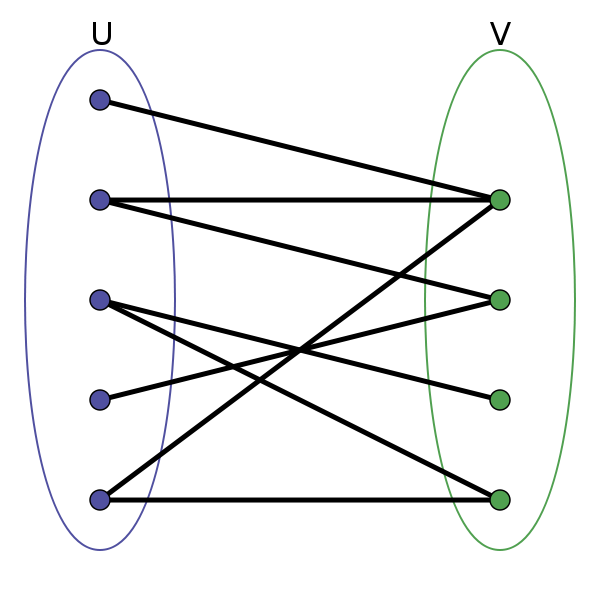
\includegraphics[width=0.4\textwidth]{Figures/bigraph.png}\centering
\end{figure}
\end{frame}

%------------------------------------------------

\begin{frame}
\frametitle{Εισαγωγικές έννοιες}
Matching\\
\begin{figure}[H]
\caption{Matching example}
\centering
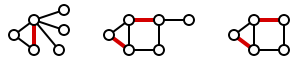
\includegraphics[width=0.6\textwidth]{Figures/match.png}\centering
\end{figure}

\begin{figure}[H]
\caption{Maximum matching example}
\centering
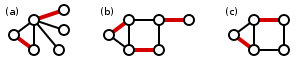
\includegraphics[width=0.6\textwidth]{Figures/max_match.png}\centering
\end{figure}
\end{frame}

%------------------------------------------------

\begin{frame}
\frametitle{Θεώρημα Konig}
Για κάθε διμερή γράφο $G=(V,E)$ ισχύει $\nu(G) = \tau(G)$ όπου\\
$\nu(G) := $ maximum size of a matching in G,\\
$\tau(G) := $ minimum size of a vertex cover in G.

\begin{figure}[H]
\caption{Maximum matching - minimum vertex cover example}
\centering
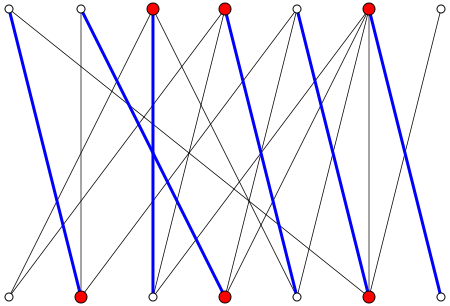
\includegraphics[width=0.4\textwidth]{Figures/KonigTheo.png}\centering
\end{figure}
\end{frame}

%------------------------------------------------

\begin{frame}
\frametitle{Απόδειξη}
Έστω ένας διμερής γράφος $G = (L, R, E)$ και ένα μέγιστο ταίριασμα $M$. Τότε επειδή κανένας κόμβος ενός vertex cover δεν μπορεί να καλύπτει περισσότερες από δύο ακμές του συνόλου $M$ (διαφορετικά δεν θα ήταν ταίριασμα), ένα vertex cover μεγέθους $|M|$ θα είναι το ελάχιστο vertex cover.\\
Για να δημιουργήσουμε ένα τέτοιο vertex cover, έστω $U$ το σύνολο των μη ταιριασμένων κόμβων του $L$, και $Z$ το σύνολο των ακμών που είτε είναι στο $U$ είτε συνδέονται με αυτό μέσω εναλλακτικών μονοπατιών (alternating paths). Τότε το σύνολο $V' = (L \setminus Z) \cup (R \cap Z)$ είναι ένα vertex cover. 
\end{frame}

%------------------------------------------------

\begin{frame}
\frametitle{Vertex Cover από Matching}
Οπότε χρησιμοποιώντας τον αλγόριθμο Hopcroft-Karp, ο οποίος βρίσκει ένα μέγιστο ταίριασμα σε ένα διμερή γράφο σε χρόνο $O(|E| \sqrt{|V|})$, μπορούμε έπειτα να υπολογίσουμε το σύνολο $V'$ αποδοτικά.
Επίσης για όλους τους γράφους ισχύει 
$$ \max_{\text{matching M}} |M| \leq  \min_{\text{vertex cover U}} |U| \leq 2 \cdot \Big( \max_{\text{mathing M}} |M|\Big)$$
\end{frame}

%------------------------------------------------
%------------------------------------------------

\subsection{Tree graphs}

%------------------------------------------------

\begin{frame}
\frametitle{Tree graphs}
Ένα δένδρο είναι ένας μη κατευθυντικός γράφος $G=(V,E)$ που είναι συνεκτικός και δεν έχει κύκλους.
Η βασική ιδέα του αλγορίθμου είναι η εξής: χρησιμοποιώντας την αναζήτηση πρώτα σε βάθος βρίσκουμε όλα τα φύλλα του δένδρου και έπειτα για κάθε φύλλο επιλέγουμε τον πατέρα του και για κάθε επιλέγουμε κάθε εσωτερικό κόμβο που τα παιδιά του δεν έχουν επιλεχθεί μέχρι να μην υπάρχουν άλλοι κόμβοι να επιλεχθούν.
\begin{figure}[H]
\caption{Tree graph vertex cover example}
\centering
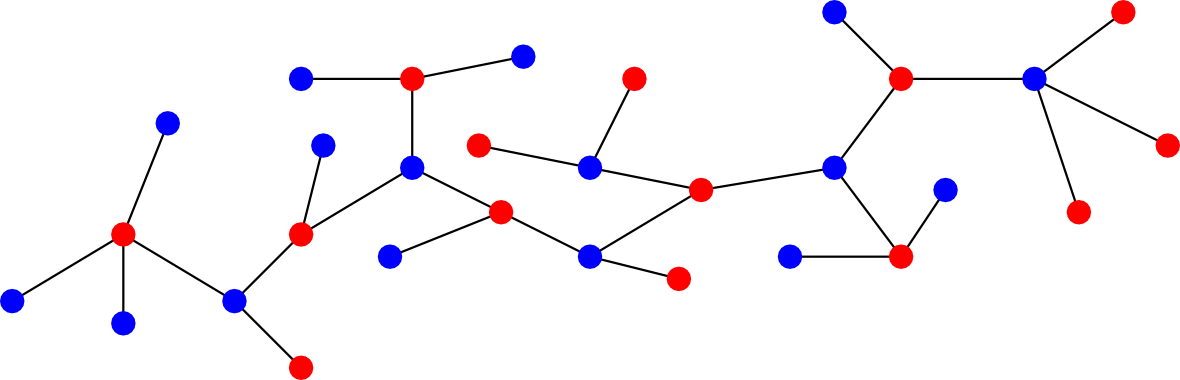
\includegraphics[width=0.4\textwidth]{Figures/vc_tree.png}\centering
\end{figure}
\end{frame}

%------------------------------------------------
%------------------------------------------------

\subsection{Δυικά προβλήματα}

\begin{frame}
\frametitle{Clique}
Ένα clique ενός μη κατευθυντικού γράφου $G=(V,E)$ είναι ένα υποσύνολο των ακμών $C \subseteq V$ τέτοιο ώστε όλοι οι κόμβοι του να είναι γειτονικοί ανά δύο.
Αν υπάρχει ένα clique $C$ στον $\overline{G}$ τότε το $V \setminus C$ είναι ένα vertex cover του $G$.\\

\begin{figure}[H]
\caption{Clique example}
\centering
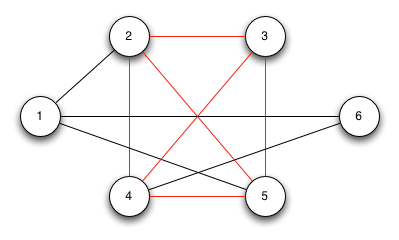
\includegraphics[width=0.4\textwidth]{Figures/VertexClique.png}\centering
\end{figure}
\end{frame}

%------------------------------------------------

\begin{frame}
\frametitle{Independent set}
Το independent set ενός γράφου είναι ένα σύνολο των κόμβων του οι οποίοι δεν είναι γειτονικοί ανά δύο.
Για κάθε independent set ενός γράφου το συμπλήρωμα του είναι ένα vertex cover για αυτόν τον γράφο.
\begin{figure}[H]
\caption{Independent set example}
\centering
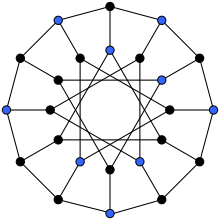
\includegraphics[width=0.3\textwidth]{Figures/indep_set.png}\centering
\end{figure}
\end{frame}

%------------------------------------------------

\section{Εφαρμογές}

\begin{frame}
\frametitle{Εφαρμογές}
\begin{enumerate}
\item Στο οδικό δίκτυο μια πόλης
\item Φύλαξη κτιρίων
\item Δυναμική ανίχνευση race conditions
\item Εξάλειψη συγκρούσεων (υπολογιστική βιοχημεία)
\end{enumerate}
\end{frame}


\begin{frame}[allowframebreaks]
\frametitle{Βιβλιογραφία}
\printbibliography
\end{frame}

\end{document} 
